\begin{pastexam}[label={px:gk3-114-ds-01}]{高考三級資訊處理 114 年 第一題}
（申論；20 分）

一棵空的階數為 3 的 B-Tree（B-Tree of order 3）。由左而右依序插入下列鍵值（key value）：10, 80, 2, 9, 45,
62。請問插入完畢後，根節點中的鍵值有那些？請依序由小到大列出，用逗號分隔，並請說明樹節點的變化。
（10 分）有一棵階數為 5 的 B-Tree（B-Tree of order 5），其高度（height）為 3，請問這棵樹中最多可以儲存
多少個鍵值？(10 分)
\end{pastexam}

\begin{pastsoln}
答案：前半題根節點的鍵值是 \textbf{10, 62}；後半題最多 \textbf{124} 個鍵值。

原卷這一題沒有印小題編號，前後兩個問題各 10 分，以下分開回答。 階數照資結書定義~11.2：$m$ 階 B 樹每個
節點最多 $m$ 個子節點、$m - 1$ 個鍵。

\textbf{前半題}。 $3$ 階 B 樹就是 2-3 樹（資結書第~11.1~節）：每個節點 $1$ 或 $2$ 個鍵。 插入時先找到
該放的葉節點、依大小放進去；節點有了 $3$ 個鍵就溢位，把中間（第 $\lceil 3/2 \rceil = 2$ 個）鍵往上送到
父節點，左右兩個鍵各自成為一個節點；根溢位時，送上去的鍵成為新的根，樹長高一層。
\begin{enumerate}[label=(\arabic*)]
\item 插入 10：空樹，建一個根 $[10]$。
\item 插入 80：放進根，$[10, 80]$，兩個鍵，沒有溢位。
\item 插入 2：放進根成 $[2, 10, 80]$，三個鍵溢位。 中間的 $10$ 上升成新的根，$2$、$80$ 分成兩個子節點：
根 $[10]$，子節點 $[2]$、$[80]$。 高度變成 $2$。
\item 插入 9：$9 < 10$，走左邊，葉節點 $[2] \to [2, 9]$。
\item 插入 45：$45 > 10$，走右邊，葉節點 $[80] \to [45, 80]$。
\item 插入 62：$62 > 10$，走右邊，$[45, 62, 80]$ 溢位。 中間的 $62$ 上升到根，根變成 $[10, 62]$，
$45$、$80$ 分成兩個葉節點。 根只有 $2$ 個鍵，不再溢位。
\end{enumerate}
最後的樹：
\begin{center}
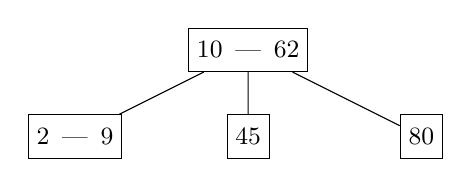
\begin{tikzpicture}[k/.style={draw,rectangle,minimum height=5.5mm,inner sep=3pt,font=\small},
    level distance=11mm, sibling distance=22mm]
\node[k] {10 \,|\, 62}
  child {node[k] {2 \,|\, 9}}
  child {node[k] {45}}
  child {node[k] {80}};
\end{tikzpicture}
\end{center}
根節點的鍵值由小到大是 \textbf{10, 62}。 檢查：三個葉節點在同一層；根有 $2$ 個鍵、$3$ 個子節點；
$[2, 9] < 10 < [45] < 62 < [80]$，符合搜尋樹的順序。

\textbf{後半題}。 $5$ 階 B 樹每個節點最多 $5$ 個子節點、$4$ 個鍵。 高度 $3$（照資結書，高度數節點的
層數，只有根的樹高度 $1$）時，要放最多鍵，就讓每個節點都滿：
\begin{center}
\small
\begin{tabular}{cccc}
\toprule
層 & 節點數 & 每個節點的鍵數 & 鍵數 \\
\midrule
1（根） & $1$ & $4$ & $4$ \\
2 & $5$ & $4$ & $20$ \\
3 & $25$ & $4$ & $100$ \\
\midrule
合計 & $31$ & & $124$ \\
\bottomrule
\end{tabular}
\end{center}
也就是資結書定理~11.1 的上界 $m^h - 1 = 5^3 - 1 = \mathbf{124}$。

如果題目的高度是數邊（只有根的樹高度 $0$，CLRS 的算法），高度 $3$ 就有 $4$ 層，最多
$5^4 - 1 = 624$ 個鍵。 國家考試的 B 樹題一般沿用數層數的定義，本書答 $124$；作答時寫出採用的高度定義。
\end{pastsoln}
